% !TEX root = ../thesis.tex

\section{Implementation}
\label{sec:implementation}
After some theoretical background information was given in the previous chapter,
the following sections aim to explain how the \gls{som} algorithm was
implemented in JavaScript. First, a smaller program was built to extend the
existing software \textit{CataRT}. Then a second, more fully
fledged application called \textit{SOM Browser} was developed. For both of
these programs, we take a look at their functionality and features, give an
overview of the code and program structure, and explain some concepts and
considerations that were important for the development process.

\subsection{Groundwork: CataRT Extension}

\begin{figure}[!htb]
  \centering
  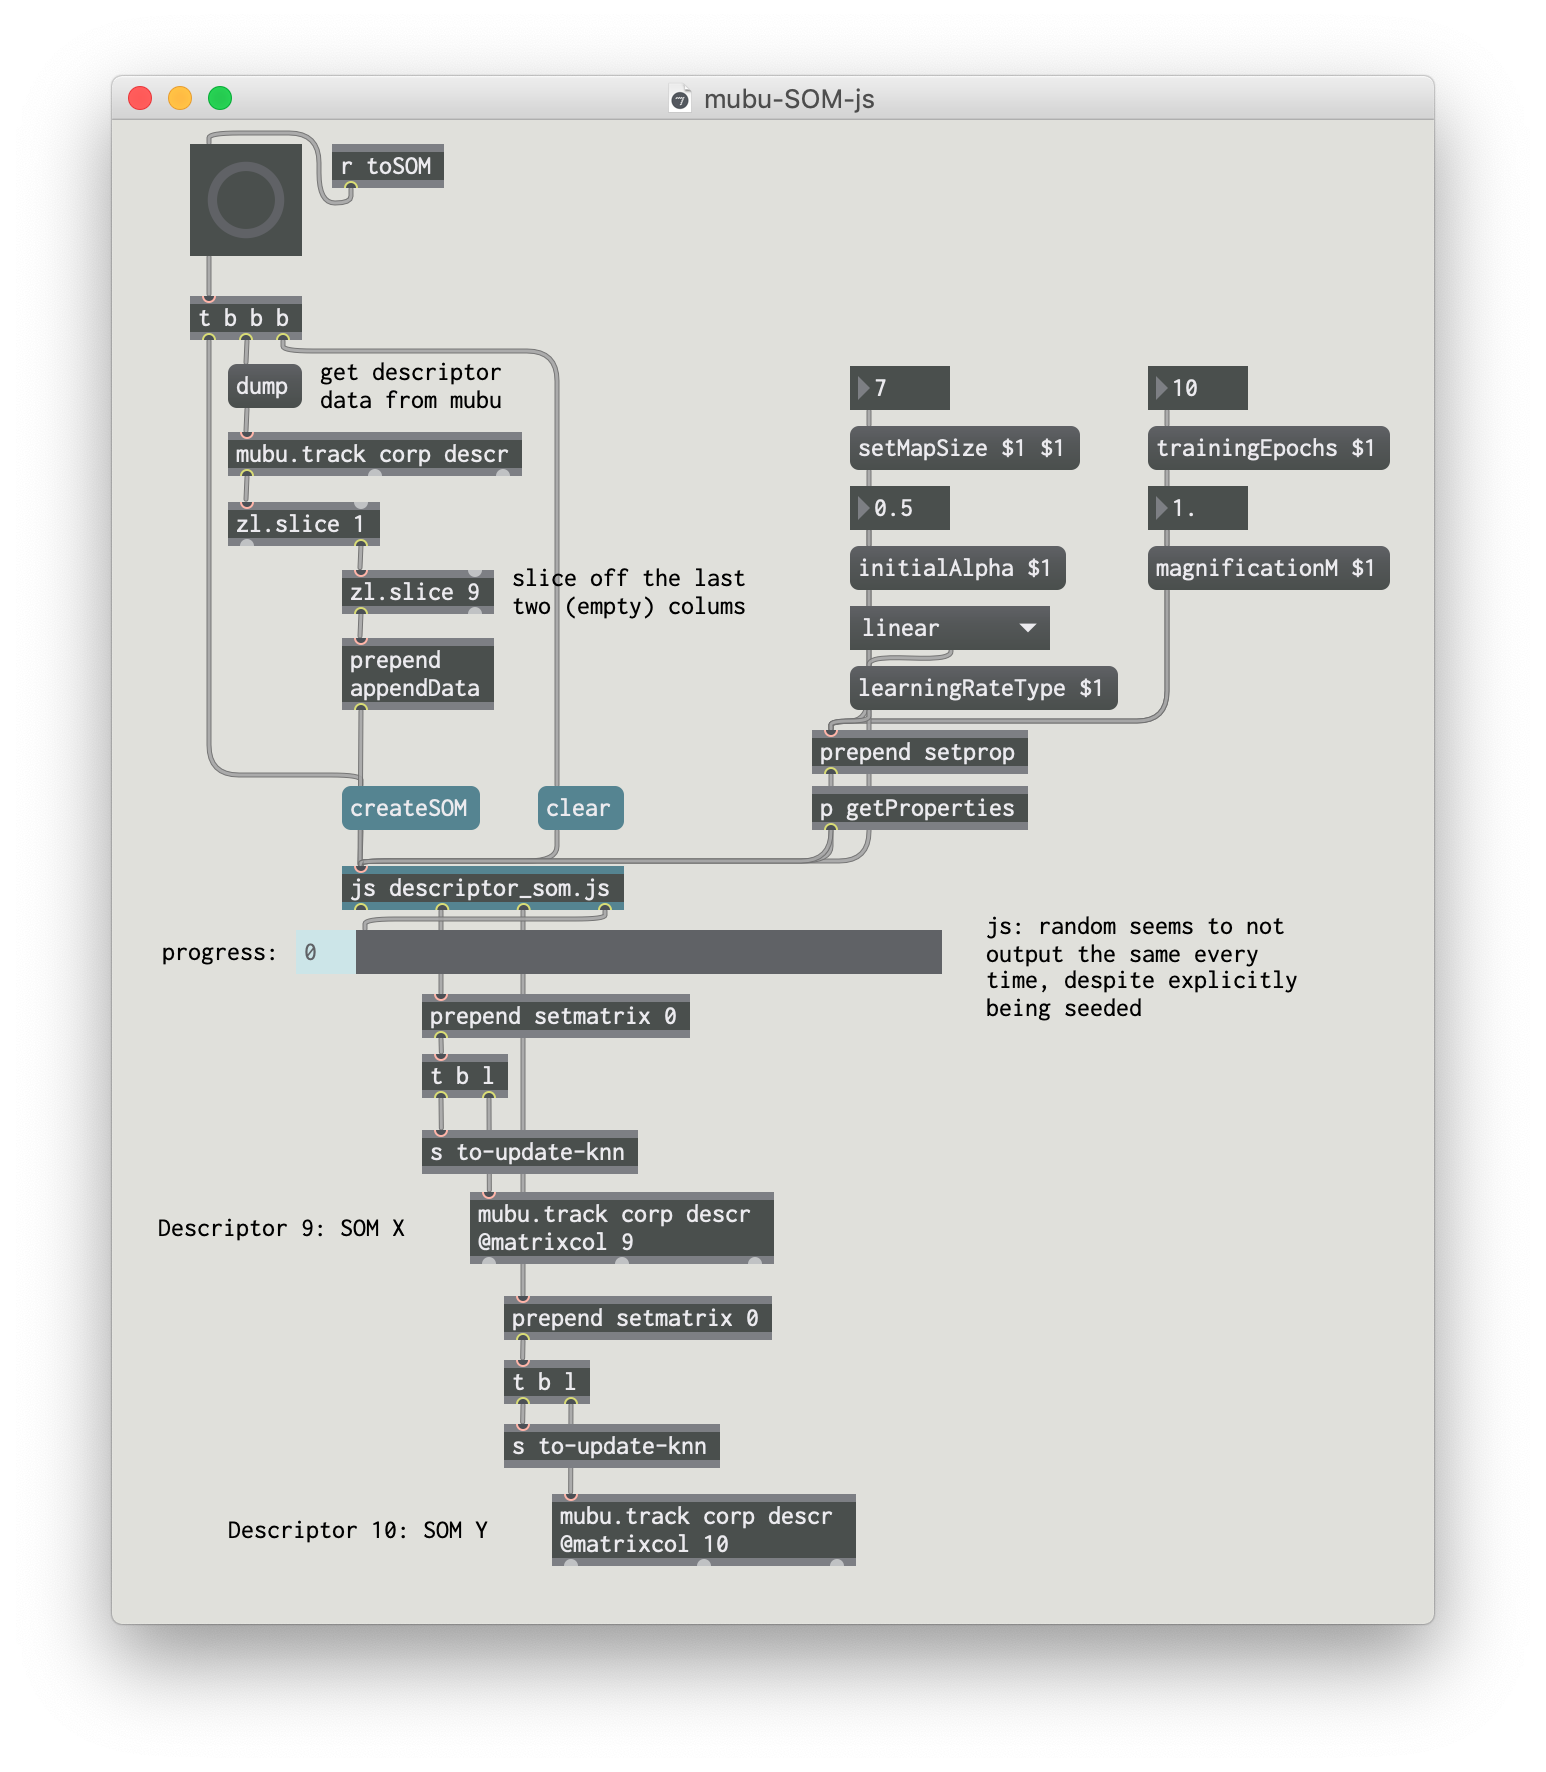
\includegraphics[width=\linewidth, clip]{mubu-som-js}
  \caption{mubu-SOM-js}
  \label{fig:mubu-som}
\end{figure}

\label{subsec:implementation_catart}
For the purpose of laying the groundwork for a bigger standalone application
(see section \ref{subsec:implementation_som-browser}), a proof-of-concept
implementation of the core \gls{som} algorithm was written in JavaScript to
serve as an extension to the \textit{MuBu For Max} software package
(\citet{web:mubu2019}, \citet{web:mubu2019_2}) for the visual programming
language Max \citep{web:max2019}. \textit{MuBu For Max} was developed by the
Sound, Music, Movement, Interaction Team (ISMM) at \gls{ircam}
\citep{schnell2009}. It contains the \textit{catart-by-mubu} patch for
realtime interactive corpus-based concatenative synthesis based on the original
\textit{CataRT} software \citep{schwarz2006}. The developed extension is a Max
patch called \textit{mubu-SOM-js} (see Figure \ref{fig:mubu-som}) and can be
found on the digital resource included with this thesis in the directory
% TODO: this
XXX path to patch XXX.

\smallskip

\begin{figure}[!htb]
% \begin{figure}
  \centering
\begin{subfigure}{0.45\textwidth}
  \centering
  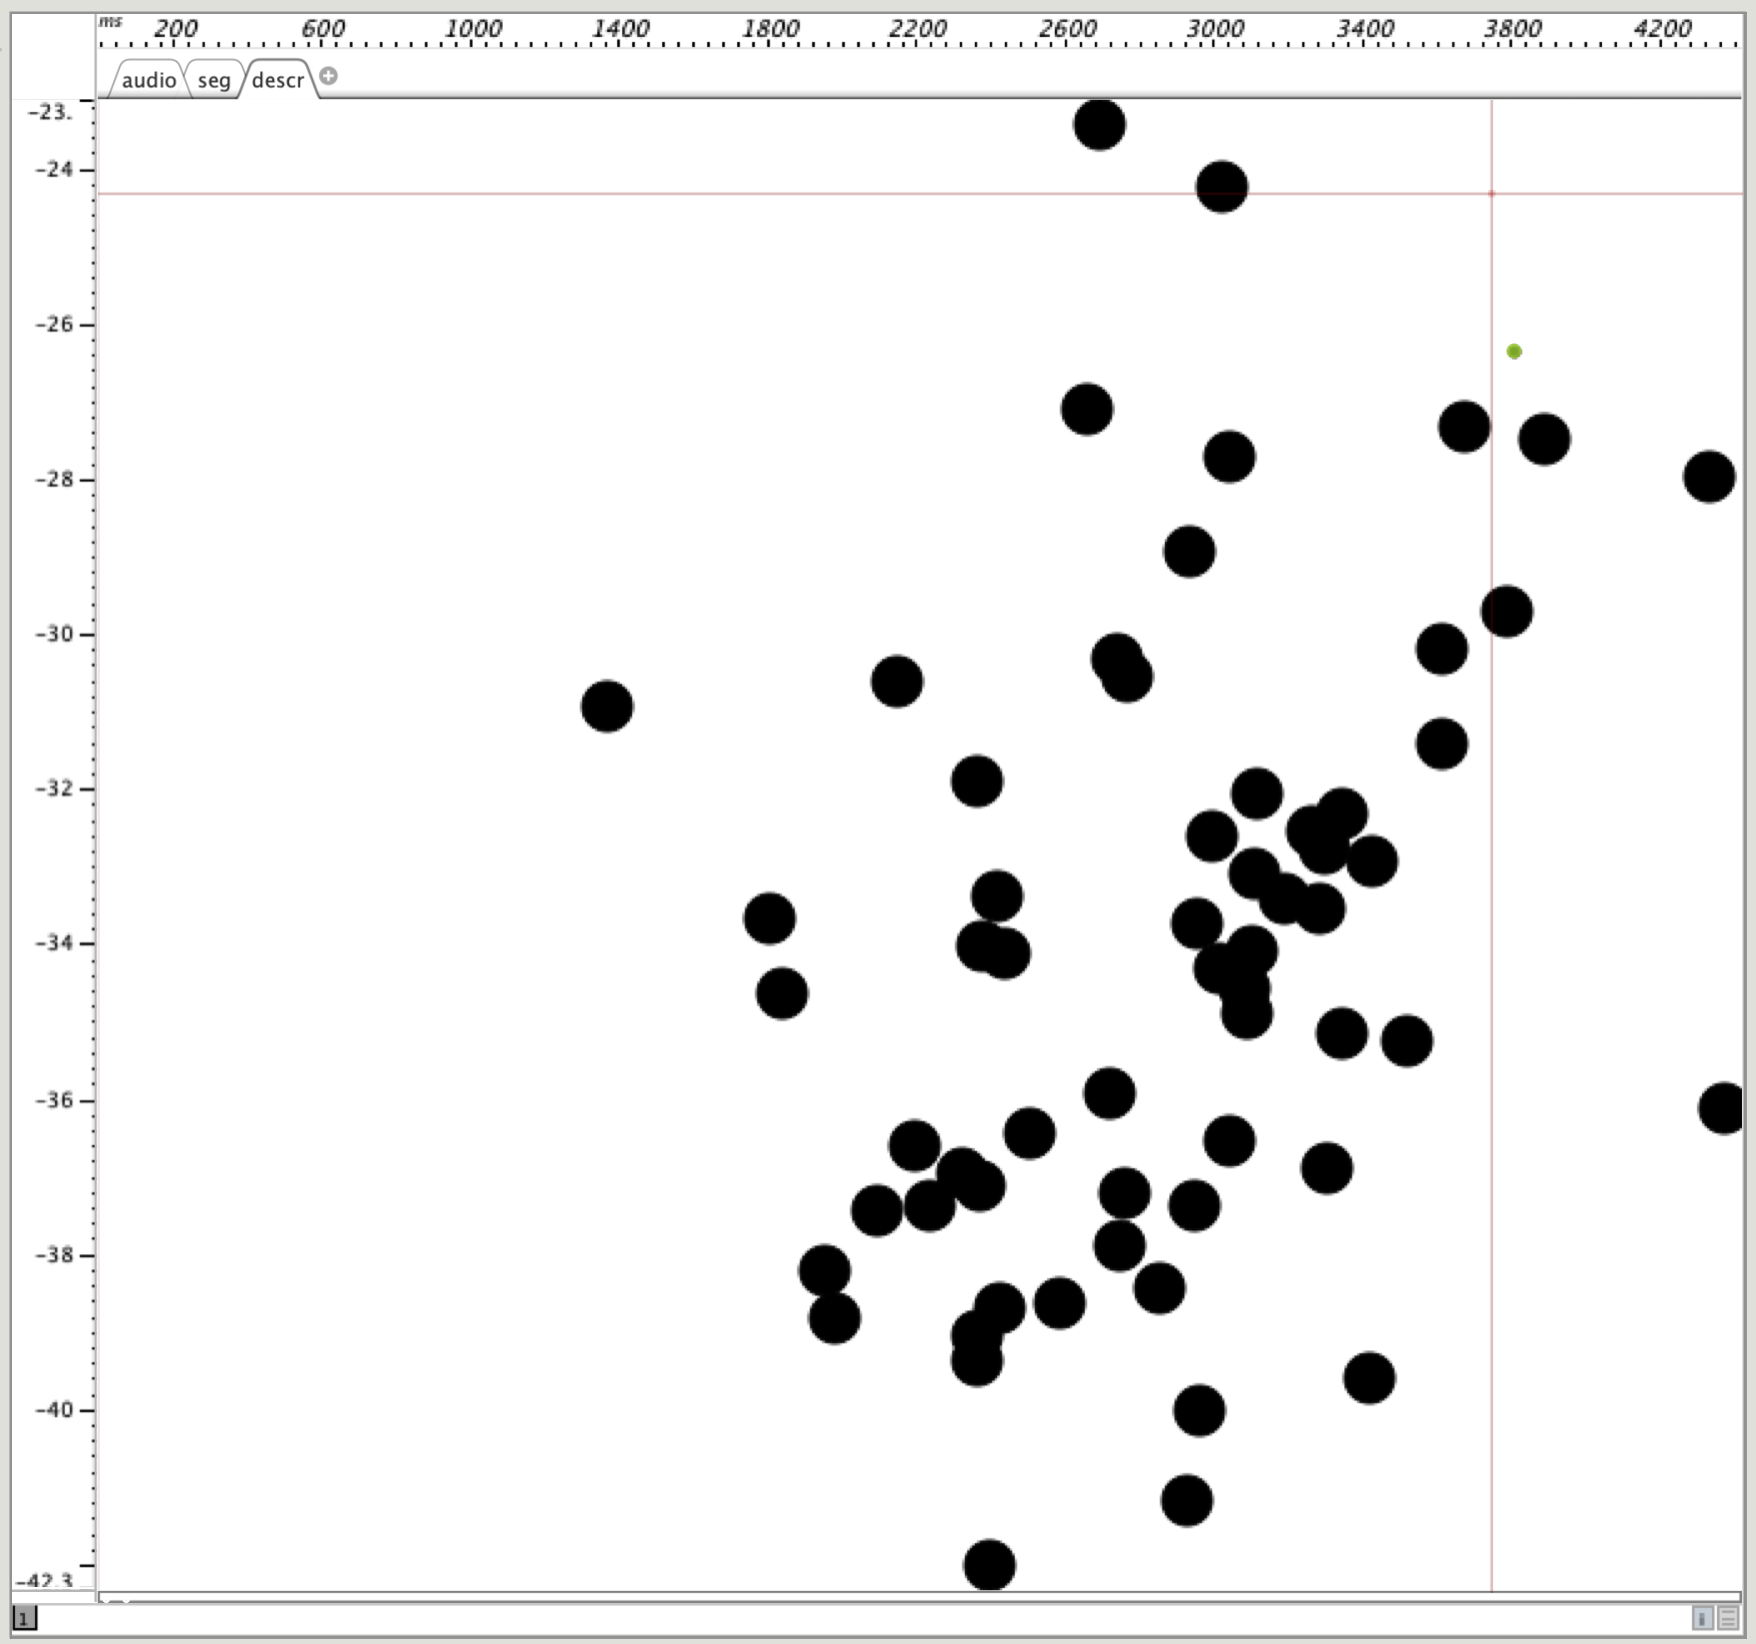
\includegraphics[width=\textwidth]{catart_without_som_centroidVSloudness}
  % \caption{\textit{CataRT} display of a corpus using spectral centroid (X axis)
  % vs loudness (Y axis)}
  \caption{}
  \label{fig:catart_no_som}
\end{subfigure}
~
\begin{subfigure}{0.45\textwidth}
  \centering
  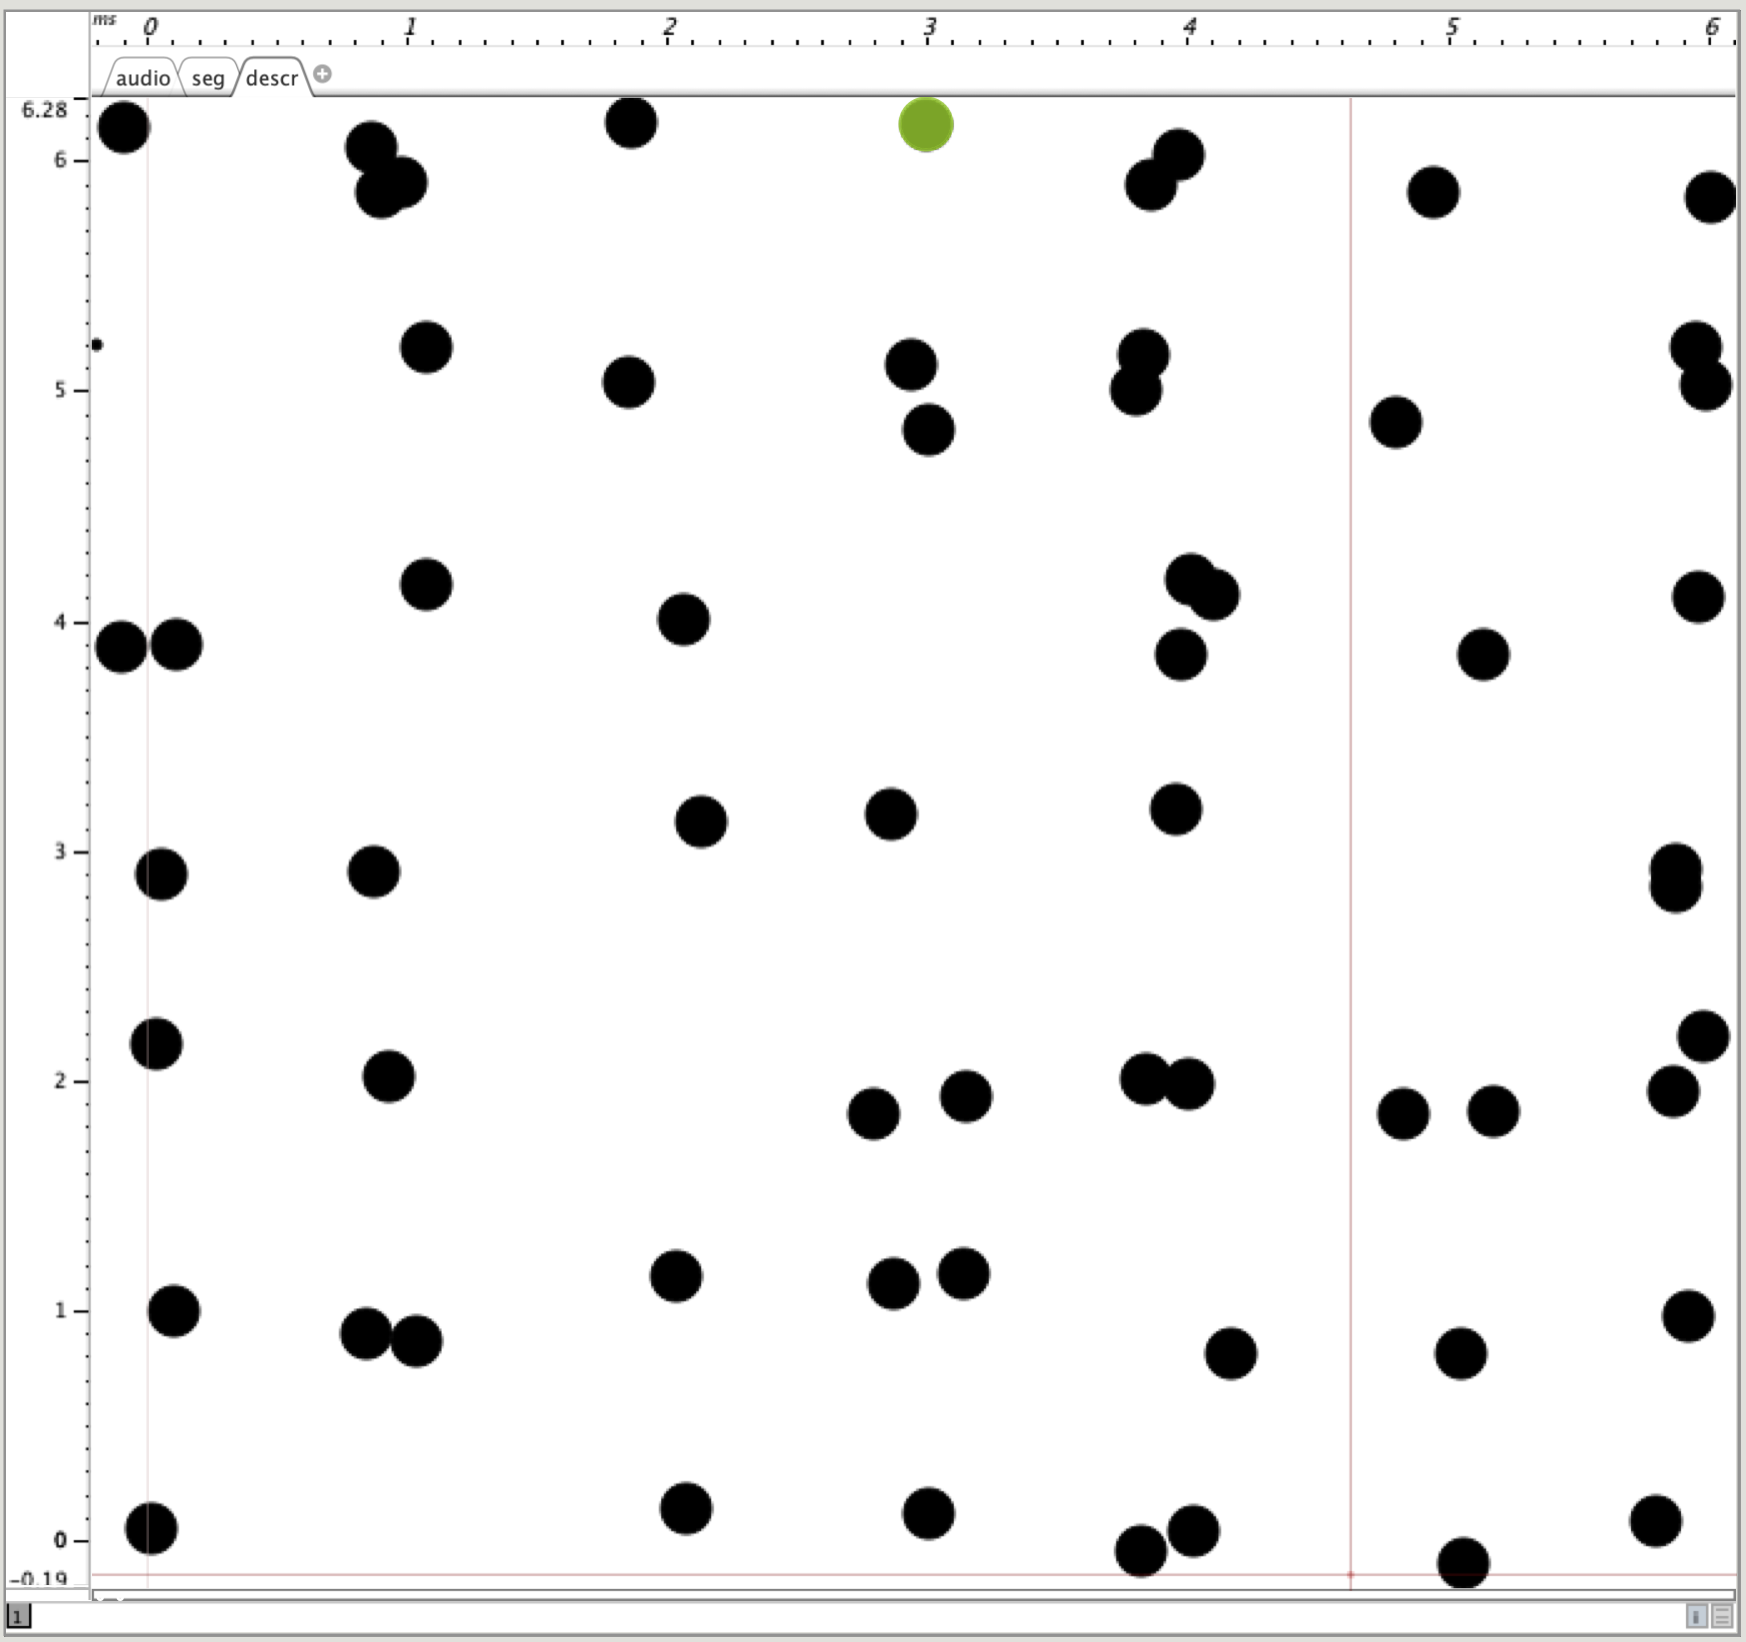
\includegraphics[width=\textwidth]{catart_with_som}
  % \caption{\textit{CataRT} display of a corpus using \gls{som} extension}
  \caption{}
  \label{fig:catart_with_som}
\end{subfigure}
\caption[\textit{CataRT}: with and without \gls{som}]{\textit{CataRT} display of
a corpus without \gls{som}
(\ref{fig:catart_no_som}, X axis shows spectral centroid, Y axis shows loudness)
and with \gls{som} extension (\ref{fig:catart_with_som}). Each circle represents
a sample.}
\label{fig:catart_som_vs_no_som}
\end{figure}


\textit{Catart-by-mubu} uses a
two-dimensional scatter plot interface in which the user can select samples or
grains from the loaded audio corpus (see Figure \ref{fig:catart_som_vs_no_som}).
The spatial position of these sounds in the interface is determined by two audio
features, representing the horizontal and vertical axes, that can be selected by
the user.
The implemented \gls{som} extension gives users the option to choose a
two-dimensional \gls{som} for the spatial organization of the corpus. This
augments the interface in three ways: all analyzed audio features can be
taken into account for the spatial positioning (as opposed to just two at a
time), more of the available interface space is used and additionally the sounds
are spaced in a more even fashion (see Figure \ref{fig:catart_som_vs_no_som}).

\subsubsection{Functionality}
\label{subsubec:mubu-som_functionality}
\textit{Mubu-SOM-js} offers the user simple controls to influence the produced
\gls{som}. These can be set by sending the messages outlined in Table
\ref{table:catart_som_messages} to the \\ \texttt{[js descriptor\_som.js]}
object.

% \paragraph*{setMapSize} takes an integer value and sets the size of the square
% map to that value.
%
% \paragraph*{trainingEpochs} defines the length of the
% training in epochs. One epoch corresponds to $n$ iterations of the training
% algorithm as defined in section \ref{subsubsec:som_math_definition}, where $n$
% is the number of samples in the corpus. Specified in integers.
%
% \paragraph*{initialAlpha} is the starting value for $\alpha$, the learning rate
% factor. It is expected to be a floating point value.
%
% \paragraph*{learningRateType} sets the learning rate type (see section
% \ref{subsubsec:som_learning_rates}). It expects a string that is either
% \mintinline{js}{'linear'}, \mintinline{js}{'inverse'} or \mintinline{js}{'BDH'}.
%
% \paragraph*{magnificationM} only applies when
% \mintinline{js}{learningRateType === 'BDH'}. It expects a floating point value
% and sets the magnification control factor $m$ (see section
% \ref{para:alpha_bdh}).

\begin{table}[!ht]
  \renewcommand{\arraystretch}{1.2}
  \centering
  \footnotesize
  \rowcolors{2}{table-bg-one}{table-bg-two}
  \begin{tabular}{ l | l | p{4.2cm} | p{3.1cm}}
    \textbf{Message} & \textbf{Type} & \textbf{Description}
    & \textbf{Example} \\
    \hline
    \texttt{createSOM} & n/a & Initiates \gls{som} calculation. &
    \texttt{createSOM} \\
    \texttt{setMapSize \$1 \$1} & Float & Sets size of map.
    & \texttt{setMapSize 7 7} \\
    \texttt{trainingEpochs \$1}
    & Int
    & Defines the length of the training in epochs. One epoch corresponds to
    $n$ iterations of the training algorithm (see section
    \ref{subsubsec:som_math_definition}), where $n$ is the number of samples in
    the corpus.
    & \texttt{trainingEpochs 30} \\
    \texttt{initialAlpha \$1}
    & Float
    & Sets the starting value for the learning
    rate factor $\alpha$.
    & \texttt{initialAlpha 0.5} \\
    \texttt{learningRateType \$1}
    & String
    & Sets the learning rate type (see section
    \ref{subsubsec:som_learning_rates}). It expects a string that is either
    \mintinline{js}{'linear'}, \mintinline{js}{'inverse'} or
    \mintinline{js}{'BDH'}.
    & \texttt{learningRateType 'linear'} \\
    \texttt{magnificationM \$1}
    & Float
    & Sets the magnification control factor $m$ (see section
    \ref{para:alpha_bdh}). Only applies when
    \mintinline[breaklines]{js}{learningRateType === 'BDH'}.
    & \texttt{magnificationM 0.02}
  \end{tabular}
  \caption{mubu-SOM-js: Messages for algorithm control}
  \label{table:catart_som_messages}
\end{table}

\subsubsection{Code Overview}
\label{subsubsec:mubu-som_overview}
The core of the \textit{mubu-SOM-js} Max patch is a JavaScript program (see the
file \texttt{mubu-som-js/descriptor\_som.js}). The choice of programming
language was determined by the fact that \textit{CataRT} is a Max patch and
JavaScript (via the built-in \texttt{[js]} object) can be used to script most
aspects of the Max environment. This JavaScript version of the \gls{som} is in
some ways a port from a first MATLAB implementation of the algorithm that was
developed by the author during an internship at \gls{ircam} in the fall of 2017.
Some aspects of the structure of the presented program are based on the
\gls{som} Toolbox that was developed at Helsinki University of Technology by
\citet{vesanto2000}.

\smallskip

The flow of the script is encapsulated in \mintinline{js}{createSOM()}.
This function calls all other important functions that make up the program, as
can be seen in Listing \ref{lst:mubu-som_create_som}.

\begin{listing}[!htb]
  \begin{mdframed}
    \inputminted[breaklines, numbers=left, firstline=34, lastline=39,
    fontsize=\footnotesize]{js}{../dev/mubu-som-js/descriptor_som.js}
  \end{mdframed}
  \caption{mubu-som-js/descriptor\_som.js: \mintinline{js}{createSOM()}}
  \label{lst:mubu-som_create_som}
\end{listing}

After data normalization and map initialization, \mintinline{js}{trainMap()} is
called, which executes the training procedure by repeatedly calling the function
\mintinline{js}{training()} in an asynchronous background process (see Listing
\ref{lst:mubu-som_training}). For each step of the training phase, all
calculations happen inside \mintinline{js}{trainingStep()}. The most important
part, the updating of node positions on each iteration, is shown in Listing
\ref{lst:mubu-som_node_updates}.


% \begin{listing}[!htb]
%   \begin{mdframed}
%     \inputminted[breaklines, numbers=left, firstline=31, lastline=32,
%     fontsize=\footnotesize]{js}{../dev/mubu-som-js/descriptor_som.js}
%   \end{mdframed}
%   \caption{mubu-som-js/descriptor\_som.js: Initialization of
%   \mintinline{js}{Task} object}
%   \label{lst:mubu-som_task}
% \end{listing}



\begin{listing}[!htb]
  \begin{mdframed}
    \inputminted[breaklines, numbers=left, firstline=203, lastline=219,
    fontsize=\footnotesize]{js}{../dev/mubu-som-js/descriptor_som.js}
  \end{mdframed}
  \caption{mubu-som-js/descriptor\_som.js: \mintinline{js}{training()}}
  \label{lst:mubu-som_training}
\end{listing}

\begin{listing}[!htb]
  \begin{mdframed}
    \inputminted[breaklines, numbers=left, firstline=306, lastline=312,
    fontsize=\footnotesize]{js}{../dev/mubu-som-js/descriptor_som.js}
  \end{mdframed}
  \caption{mubu-som-js/descriptor\_som.js: neuron position updates inside
  \mintinline{js}{trainingStep()}}
  \label{lst:mubu-som_node_updates}
\end{listing}

\smallskip

After the training phase is finished, the final map is populated by iterating
over all vectors and finding their corresponding best matching units (meaning
that node which is closest), as can be seen in Listing
\ref{lst:mubu-som_find_bmus}. In order to spatially differentiate between
vectors that were assigned to the same node, a small amount of random noise is
added to the position. This creates clusters around the exact node position and
allows for the individual circles to be selected. An example of a map without
added noise can be found in Figure \ref{fig:catart_with_som_no_noise}.

\begin{listing}[!htb]
  \begin{mdframed}
    \inputminted[breaklines, numbers=left, firstline=316, lastline=335,
    fontsize=\footnotesize]{js}{../dev/mubu-som-js/descriptor_som.js}
  \end{mdframed}
  \caption{mubu-som-js/descriptor\_som.js: \mintinline{js}{findBestMatches()}}
  \label{lst:mubu-som_find_bmus}
\end{listing}

\begin{figure}[!htb]
  \centering
  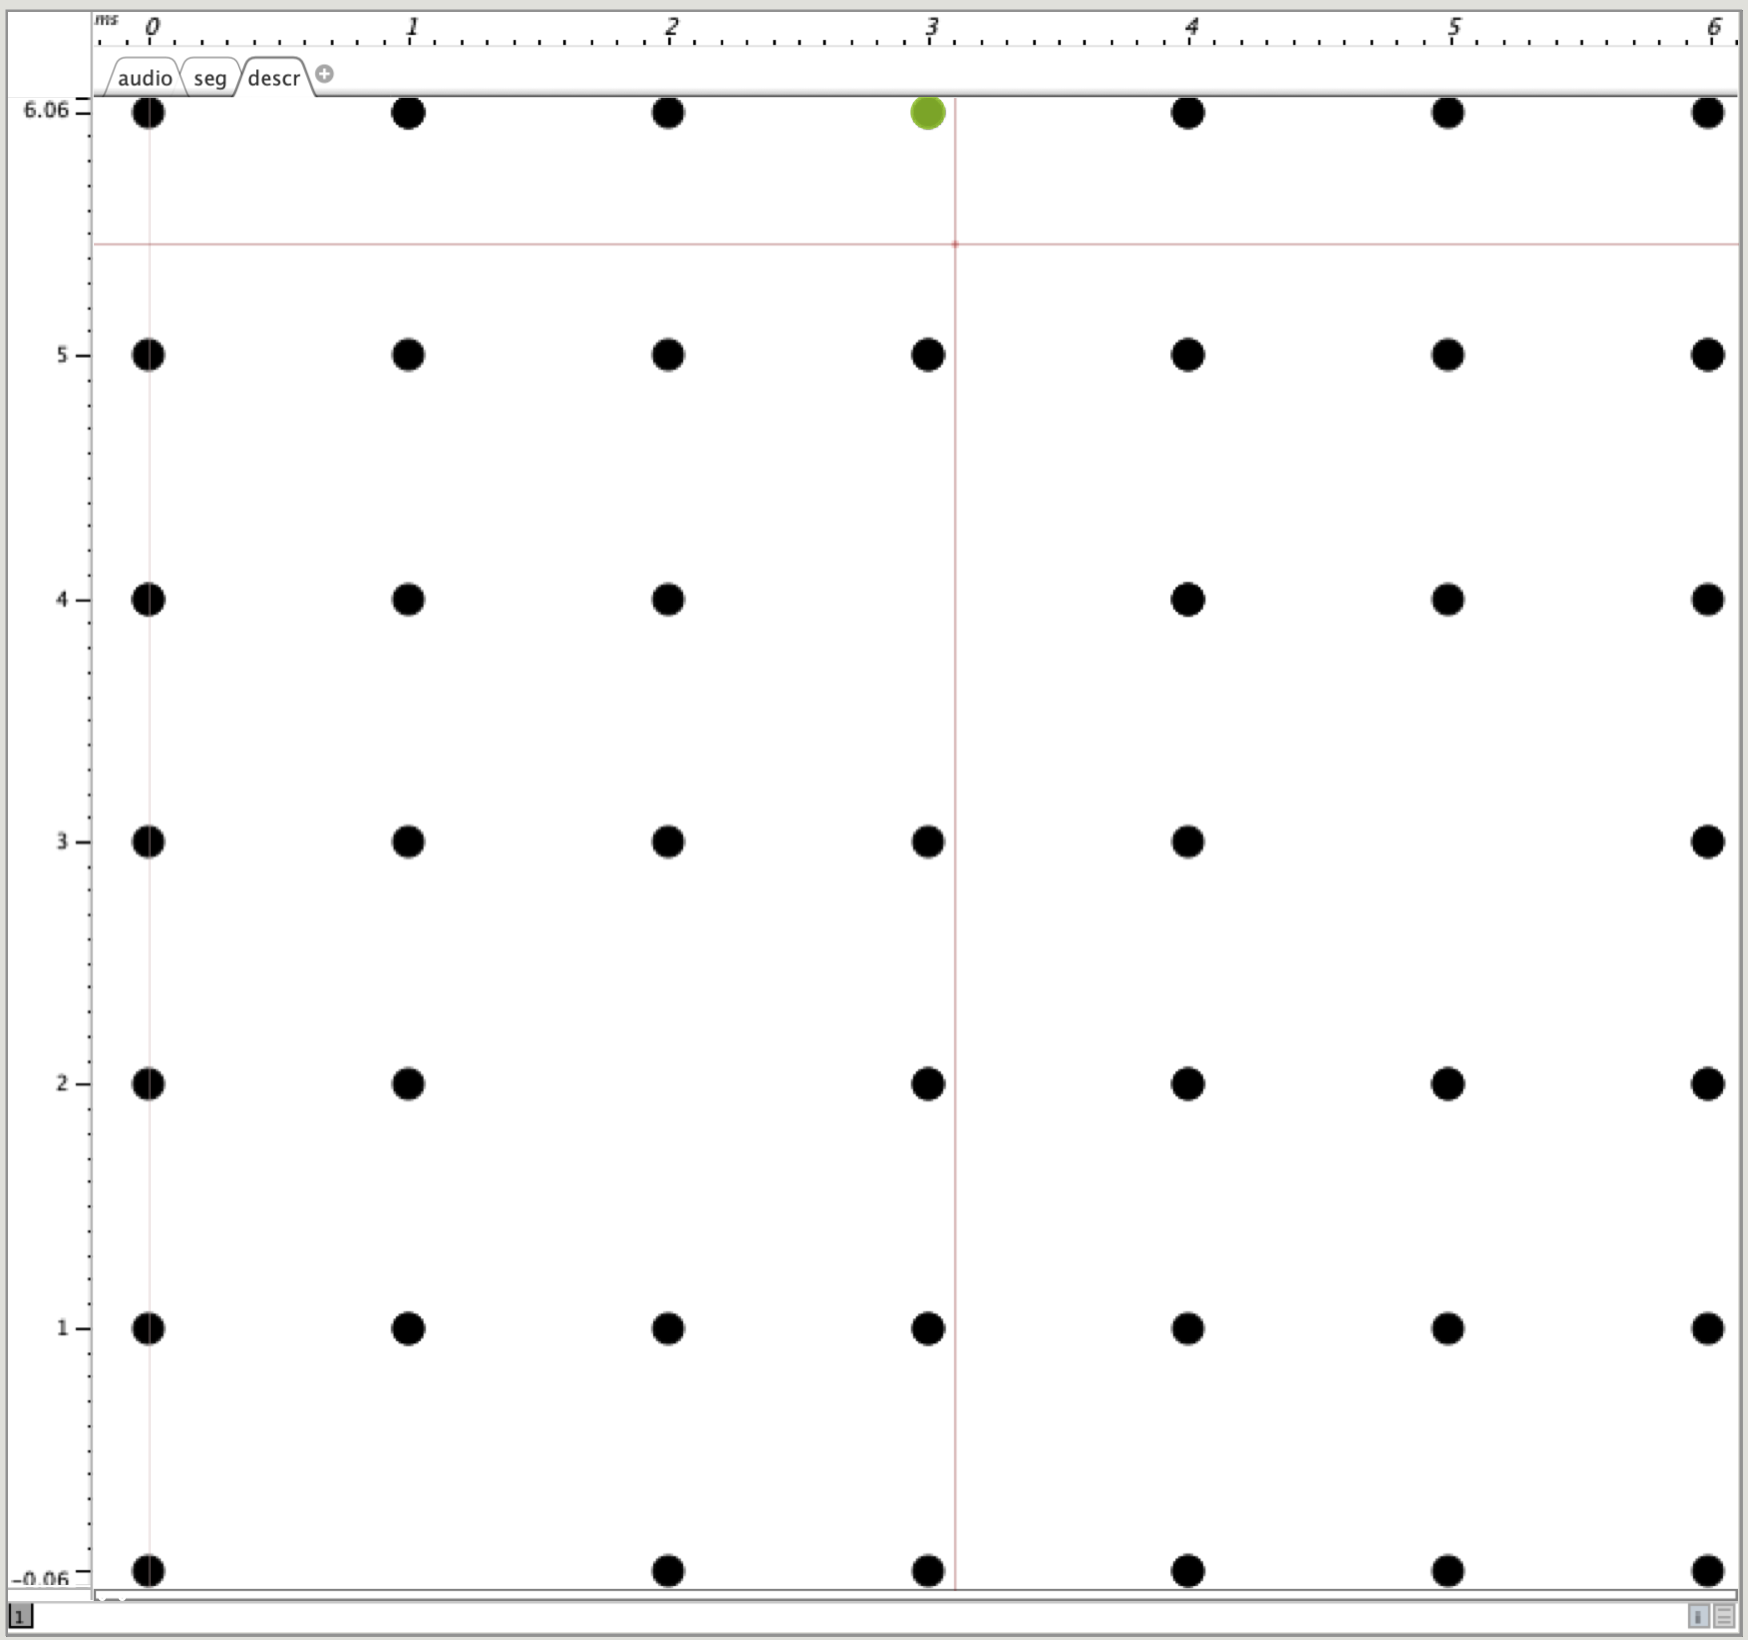
\includegraphics[width=0.45\linewidth]{catart_with_som_no_noise}
  \caption[\textit{CataRT}: \gls{som} without added noise ]{\textit{CataRT}
  display of a corpus with \gls{som} extension, but without added noise to
  differentiate samples assigned to the same node. Each circle represents a
  sample.}
  \label{fig:catart_with_som_no_noise}
\end{figure}



\clearpage

\subsection{SOM Browser}
\label{subsec:implementation_som-browser}

The majority of the work for this thesis consisted of the development of a
standalone application for sample library exploration which we call
\textit{SOM Browser}. A screenshot of the program can be seen in Figure
\ref{fig:som-browser}.

\begin{figure}[!htb]
  \centering
  \makebox[\textwidth][c]{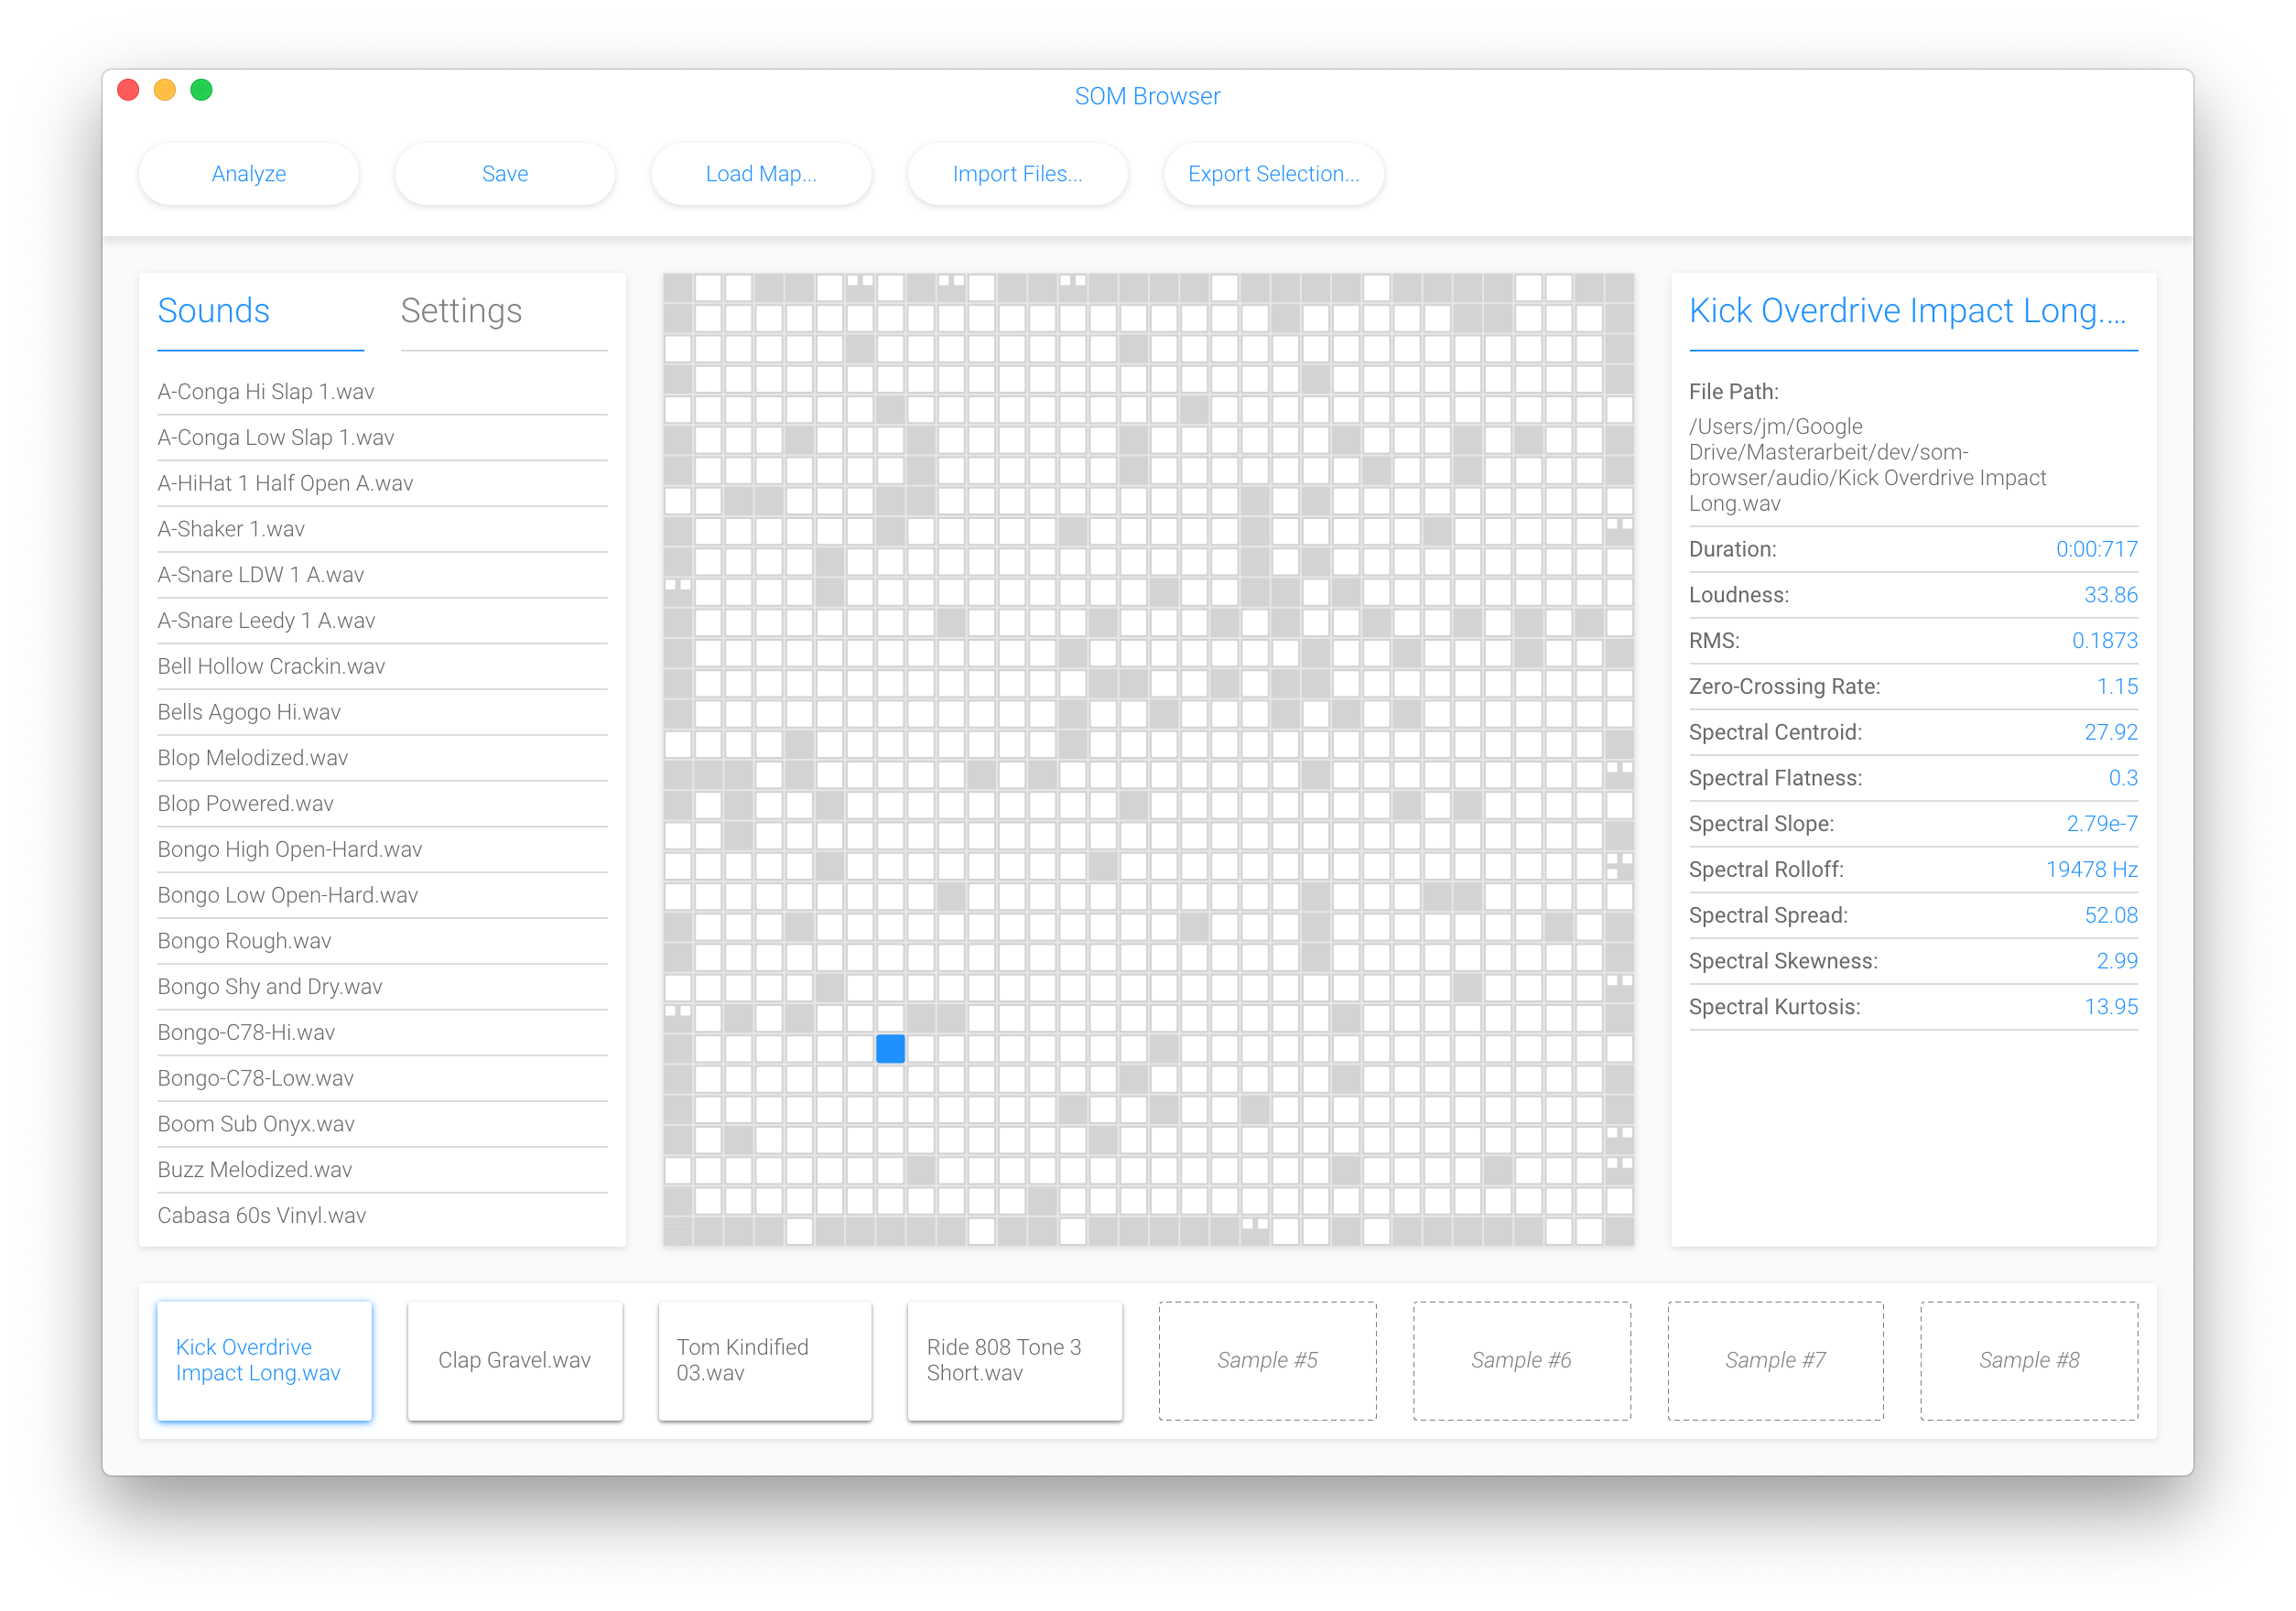
\includegraphics[width=1.4\textwidth]{SOM-Browser}}
  \caption{\textit{SOM Browser}}
  \label{fig:som-browser}
\end{figure}

\textit{SOM Browser} offers users an alternative interface for the interaction
with a folder of audio samples. Instead of the traditional file browser
interface consisting of an alphabetical list of file names, the presented
application offers a spatial map layout of the samples, with the aim of allowing
users a more direct interaction and giving them a quicker overview of the
sounds.

\subsubsection{Functionality}
\label{subsubsec:som-browser_functionality}
\paragraph{Loading Audio Files}
When launching \textit{SOM Browser}, the application opens with no sounds or map
loaded (see Figure \ref{fig:som-browser_empty}). In order to create a map of
a collection of sound files, the user can go to the menu bar at the top of the
window and click the \textit{"Import Files..."} button to load several audio
files.

\begin{figure}[!htb]
  \centering
  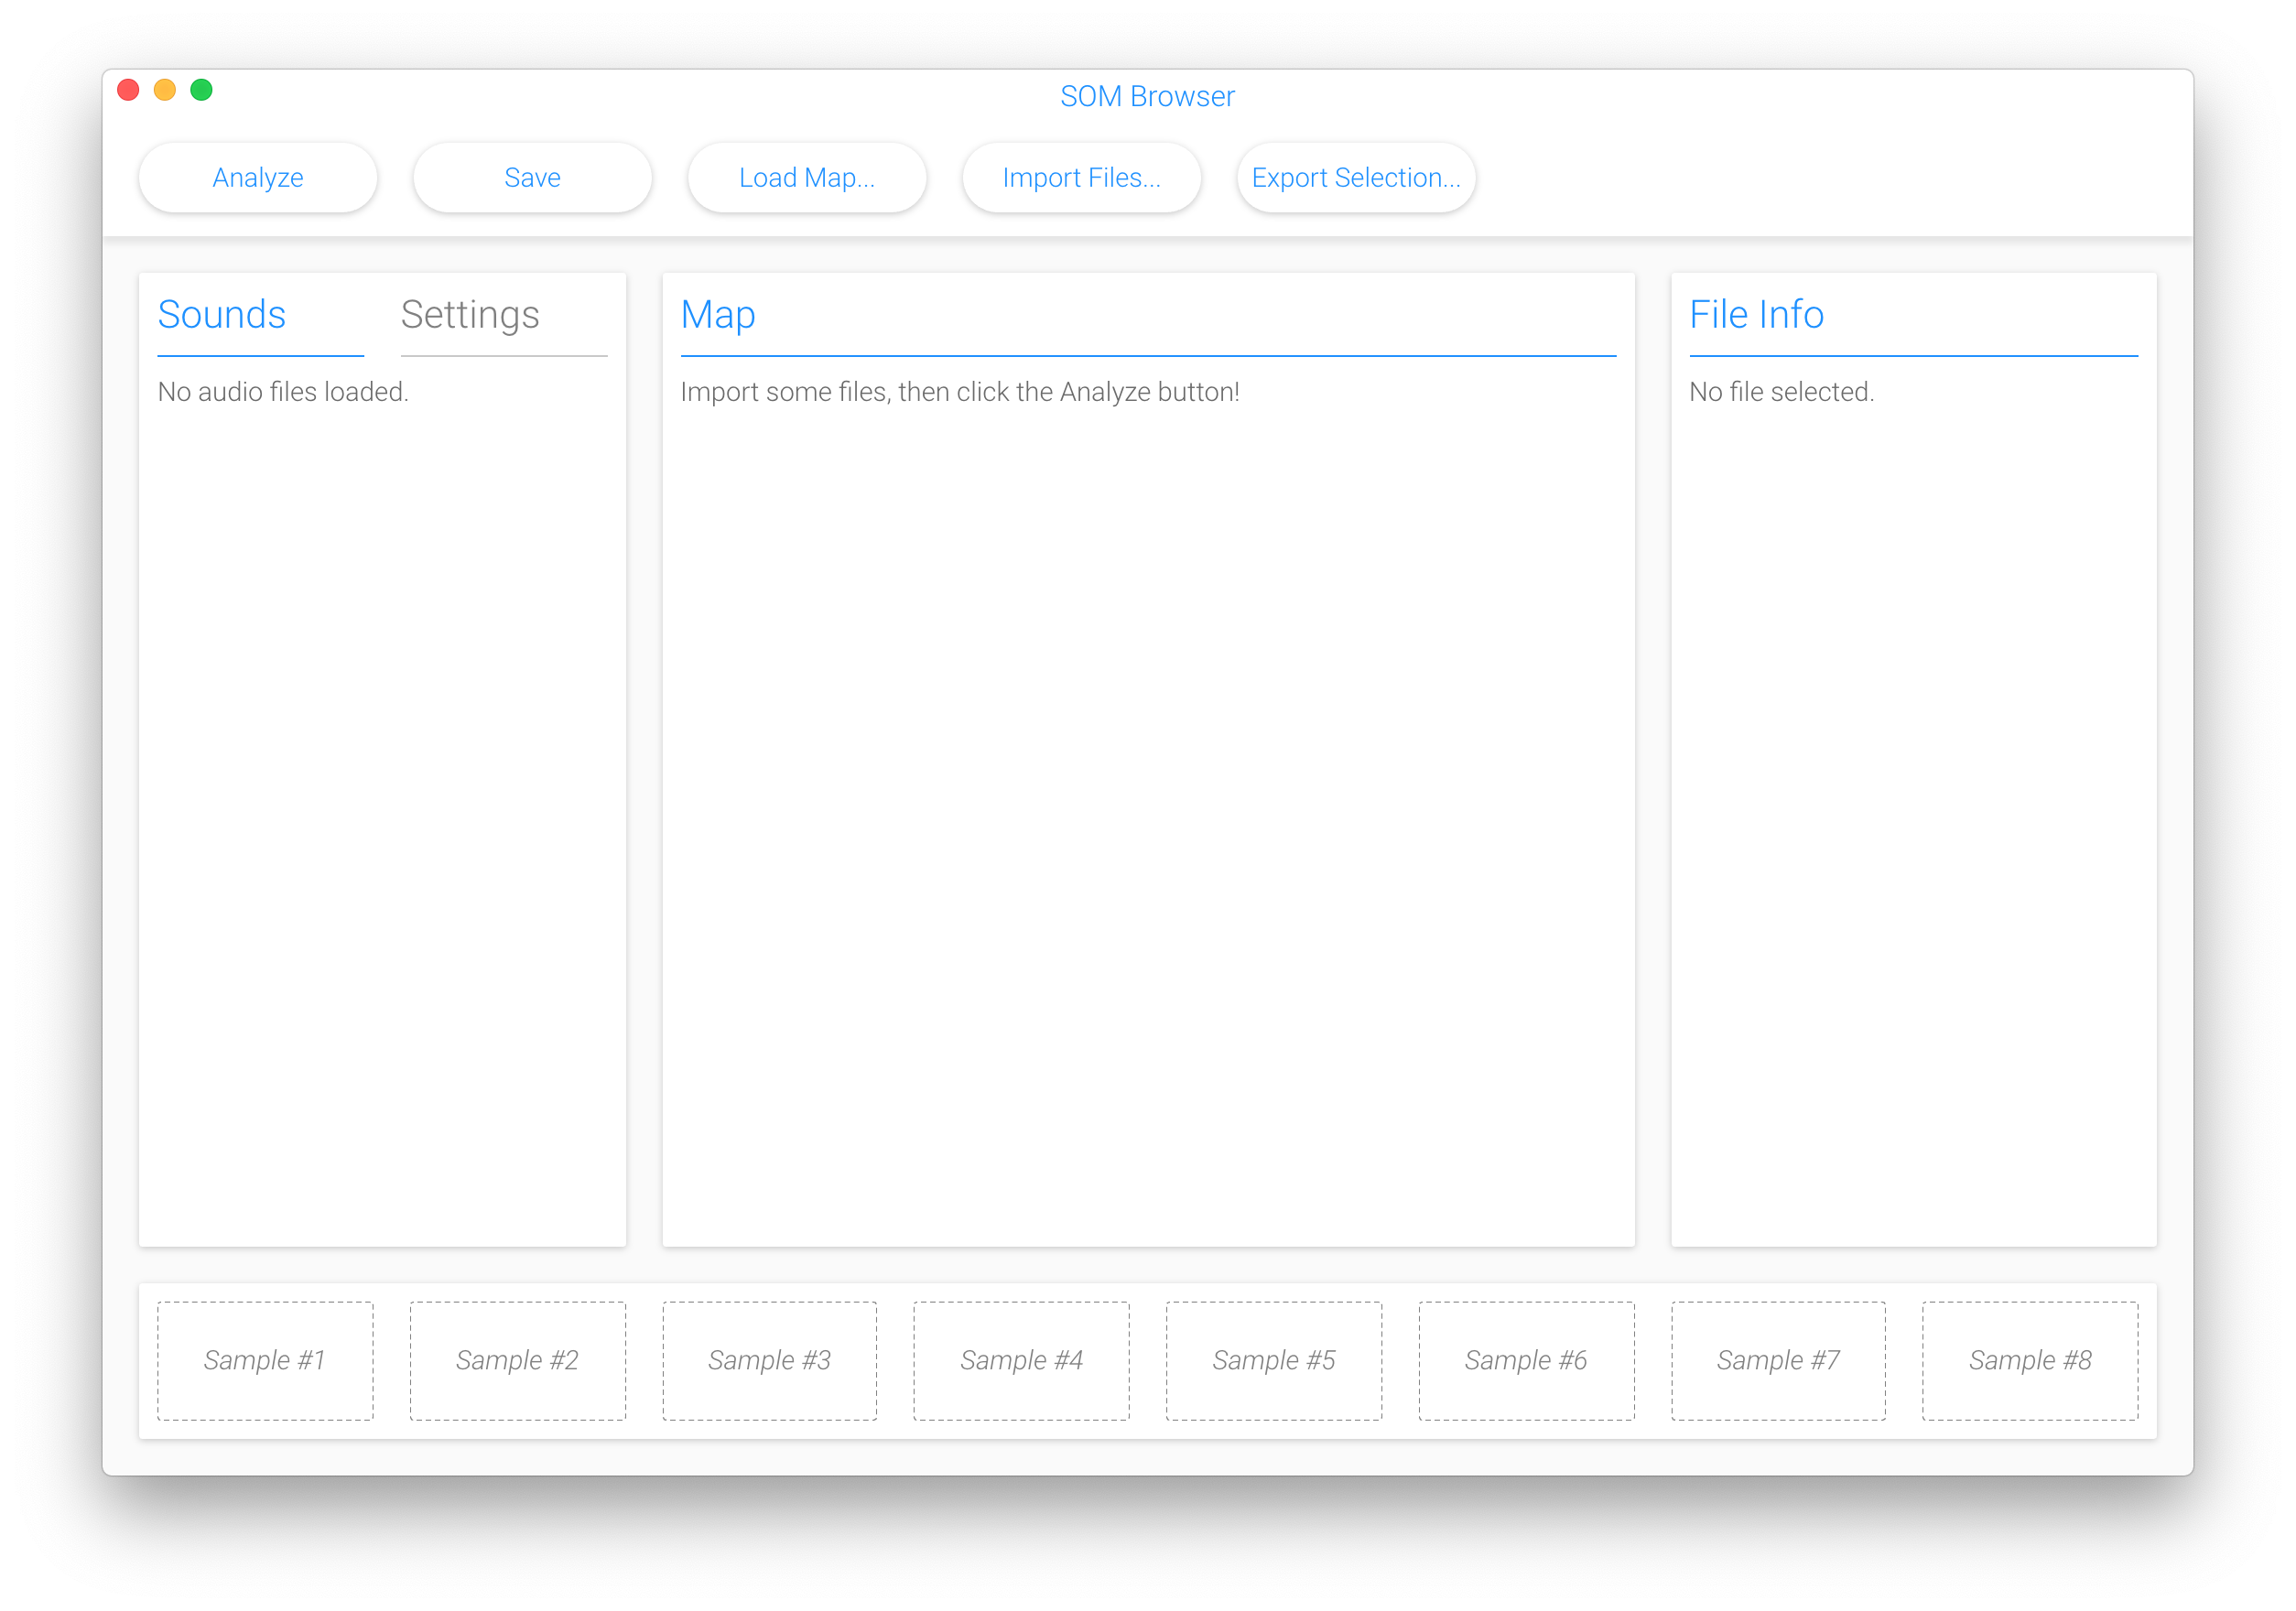
\includegraphics[width=0.7\textwidth]{SOM-Browser_empty}
  \caption{\textit{SOM Browser} without audio files loaded}
  \label{fig:som-browser_empty}
\end{figure}

\paragraph{Calculating a Map}
Once files are selected, the \textit{Sounds} list on the left side of the
application will be populated. Next, by clicking \textit{"Analyze"}, the program
will start to analyze the audio files in the background, first extracting
audio features (see section \ref{subsec:feature_extraction}) and then using this
information to calculate a \gls{som} using default settings. Alternatively,
some \gls{som} parameters can be altered by selecting the \textit{Settings}
field next to \textit{Sounds} and adjusting the exposed parameters. Depending on
the number of audio files to analyze and the selected training duration, the
algorithm will take a while to process. Training progress is indicated as a
percentage in the central \textit{Map} panel.

\smallskip

\paragraph{Map Interaction}
Upon completion of the \gls{som} calculation, the \textit{Map} panel will be
populated by a grid of white and grey squares. Each white square represents a
single sound file. All files are loaded into the computer's \gls{ram} for quick
access. Grey squares are empty nodes, meaning nodes to which no sound
files were assigned. Sounds can be played by clicking on the white squares.
They can also be played immediately by holding down the Shift key and hovering
over them.
This allows the user a very fast audition process and makes it
possible to play back many files in fast succession, enabling very quick
browsing of all loaded audio files. When hovering over a square, the
corresponding file name is shown next to the mouse cursor. More detailed
information about the file, including its full path, duration and audio feature
values can be found in the \textit{FileInfo} panel to the right of the map.

\paragraph{Selecting and Exporting Favorites}
The bottom of the window is taken up by the \textit{Favorites} bar. If a sample
is found on the map that the user would like to save for further usage, they can
drag the square from the map down into one of the slots labeled
\textit{"Sample \#1 - \#8"}. Samples can also be also be played from the
\textit{Favorites} bar by clicking on them. If the user is satisfied with their
selection of samples, they can export the selected \textit{Favorites} (e.g. for
further usage in a \gls{daw}) by clicking on \textit{"Export Selection"} in the
top menu bar. This will open a file dialog window to select a location where the
files should be stored.

\paragraph{Saving and Loading Maps}
\textit{SOM Browser} also offers the ability to save entire maps to disk for
recall in a later session or import previously stored maps by clicking on the
menu bar buttons \textit{"Save"} and \textit{"Load Map"}.

\subsubsection{Libraries and Frameworks Used}
\label{subsubsec:som-browser_libraries}
Although a desktop application, \textit{SOM Browser} was built entirely using
web technologies, most importantly JavaScript. A vast variety of libraries and
frameworks are available to use for all aspects of the development process.
The following paragraphs outline the tools chosen for this application and their
benefits.

\paragraph{Electron}
\label{para:electron}
"is an open source library developed by GitHub for building cross-platform
desktop applications with HTML, CSS, and JavaScript. Electron accomplishes this
by combining Chromium and Node.js into a single runtime and apps can be
packaged for Mac, Windows, and Linux" \citep{electron2019}. It offers a variety
of \glspl{api} to offer native menus, interact with the file system and more.
Its \texttt{ipcMain} and \texttt{ipcRenderer} \glspl{api} are used for
asynchronous communication between the \gls{gui} and processes running in the
background.

\paragraph{React}
\label{para:react}
is a JavaScript library for building user interfaces \citep{react2019}. It
breaks the \gls{gui} into smaller, self-contained units called
\textit{components} that can be independently updated and rendered.

\paragraph{Web Audio API}
\label{para:web_audio_api}
enables audio processing and synthesis in (web) applications
\citep{webaudio2019}. The use of this \gls{api} makes it possible to write all
audio processing code for the presented work in JavaScript. Its core concept is
the \textit{audio routing graph}, made up of \textit{audio nodes} (simple
building blocks such as an oscillator or a recording). This graph connects
sources to other other nodes (e.g. effects or filters) and finally to an output
destination.

\paragraph{Meyda}
\label{para:meyda}
"is a Javascript audio feature extraction library. Meyda supports both offline
feature extraction as well as real-time feature extraction using the Web Audio
API" \citep{web:meyda2019}. Its effectiveness has been validated by researchers
at Queen Mary University ("Meyda [...] provide[s] excellent real time feature
extraction tools", \citet{moffat2015}).

\subsubsection{Application Structure}
\label{subsubsec:som-browser_structure}
\textit{SOM Browser} is a \textit{stateful} application, meaning it is designed
to remember user interactions, save its internal data (the \textit{state} of
the application) between interaction steps and to allow the storing of state
data between sessions.

\paragraph{System States}
\label{para:som-browser_states}
Before the start of the development process, a set of system states was designed
to represent the states through which the application is supposed to progress.
These states and their order are shown in Figure \ref{fig:som-browser_states},
giving an abstract overview of the flow of the program. Each panel represents
a state and consists of a title (shown in capitalized words at the top, e.g.
\textit{Map Created}), a method describing a state transition (underscored and
in lower case, e.g. \textit{show map}) and the next state to transition into
(bottom right, marked by an arrow, e.g. $ \rightarrow $ \textit{File Audition}).

\begin{figure}[!htb]
  \centering
  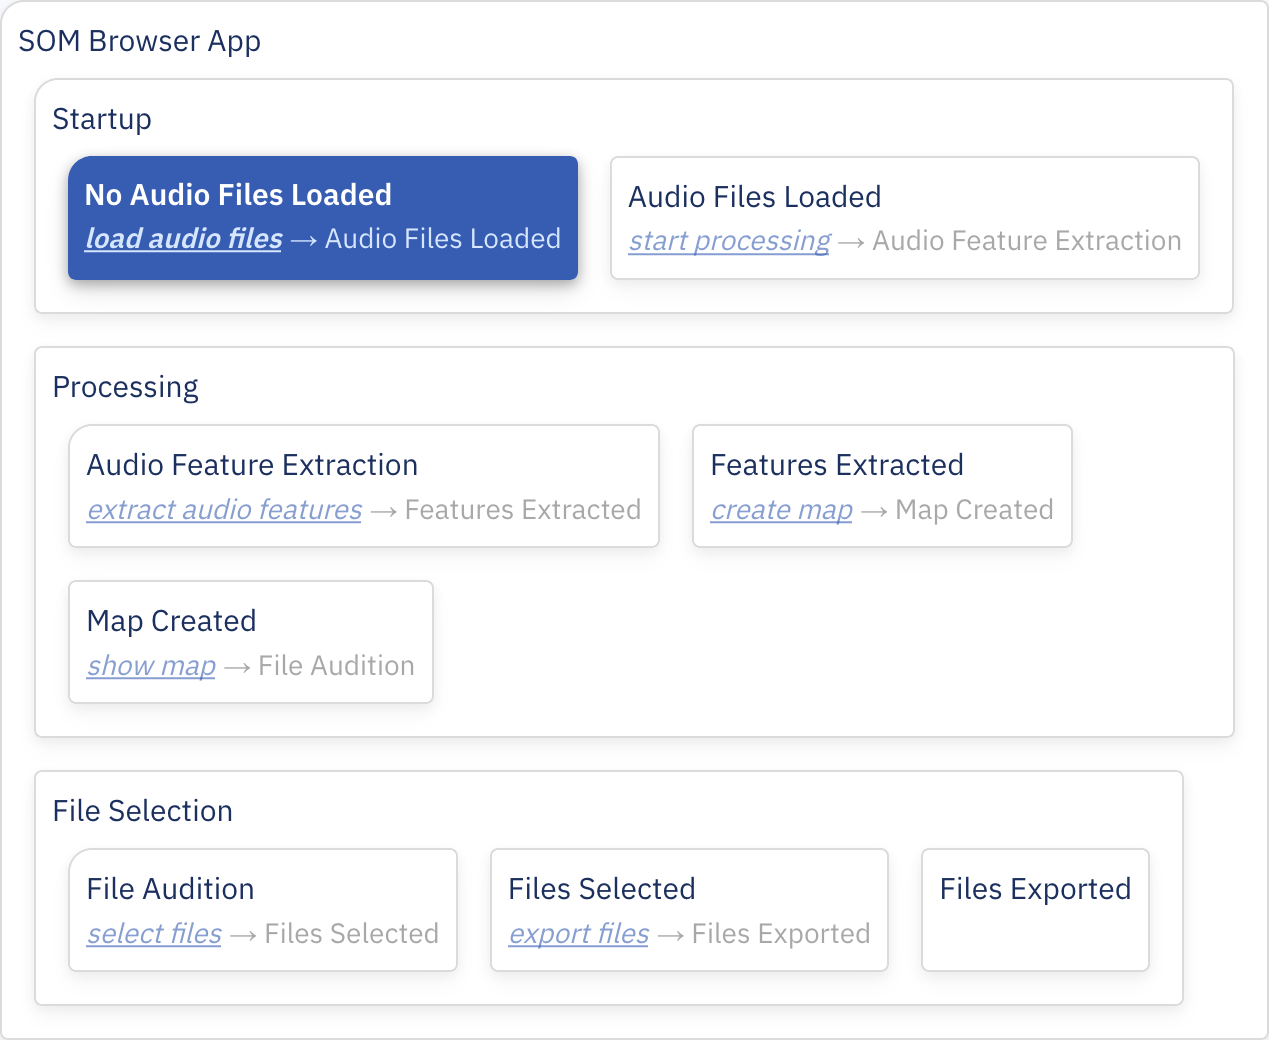
\includegraphics[width=\textwidth]{som-browser_states-sketch}
  \caption{\textit{SOM Browser}: Mock-up outlining system states}
  \label{fig:som-browser_states}
\end{figure}

\paragraph{Code Overview}
\label{para:som-browser_overview}
\textit{SOM Browser} was developed using the \textit{git} version control
system \citep{git2019} in a repository on GitHub \footnote{\href
{https://github.com/jonasmargraf/som-browser}
{https://github.com/jonasmargraf/som-browser}}.
The very basic structure of the application, in particular the way in which the
Electron and React frameworks interact, is based on a boilerplate project by
Phillip Barbiero \citep{barbiero2017}.

\smallskip

The entry point of any Electron application is the \texttt{main.js} file, which
in the presented work can be found in \texttt{som-browser/src/main.js}.
This file creates an instance of the \mintinline{js}{BrowserWindow} class called
\mintinline{js}{mainWindow} that serves as the single visible application
window. \mintinline{js}{mainWindow} then loads
\texttt{som-browser/src/index.js}, which imports the React library and uses the
React function \mintinline{jsx}{render()} to create the
\mintinline{jsx}{<App />} component, which is defined in
\texttt{som-browser/src/components/App.js}. It serves as a container for the
rest of the application logic and the entire \gls{gui} (see Listing
\ref{lst:som-browser_app_content} and Section
\ref{subsubsec:som-browser_components} for more details).
From here, the structure of the source files branches out into the individual
\gls{gui} elements in \texttt{som-browser/src/components/} and a set of files in
\texttt{som-browser/src/background/} containing the code for audio feature
extraction and \gls{som} calculation.

\subsubsection{Background Processing}
\label{subsubsec:som-browser_background_processing}
Both audio feature extraction and \gls{som} calculation are processing intensive
tasks, therefore it was clear from the beginning of the development stage that
these parts of the application must be separated from the \gls{gui} that the
user interacts with. While it is not possible to built a truly multithreaded
application (due to the fact that the fundamental Node.js framework is single
threaded), one can create separate processes to run different tasks
asynchronously. This is done by creating multiple \mintinline{js}{BrowserWindow}
instances, as each window is running in its own process. These windows can have
their \mintinline{js}{show} flag set to \mintinline{js}{false} in order to hide
them, thereby creating an invisible window for a background process.

\smallskip

\textit{SOM Browser} initiates two consecutive background processes when the
user clicks on \textit{"Analyze"}, one for feature extraction and one that runs
the \gls{som} algorithm. This is handled by the function
\mintinline{jsx}{handleAnalyzeClick()} in
\textit{som-browser/src/components/App.js}, which passes the necessary data to
these background processes by calling \mintinline{js}{processFiles(files)} and
\\ \mintinline{js}{createSOM(files, settings)} (see Listing
\ref{lst:som-browser_analyze}). Note the chaining of commands using several
\mintinline{js}{.then()} statements: \textit{SOM Browser} performs asynchronous
operations using the \mintinline{js}{Promise} feature of ECMAScript 2015
\footnote{\href{https://developer.mozilla.org/en-US/docs/Web/JavaScript/Reference/Global\_Objects/Promise}
{https://developer.mozilla.org/en-US/docs/Web/JavaScript/Reference/ \\
Global\_Objects/Promise}}.

\begin{listing}[!htb]
  \begin{mdframed}
    \inputminted[breaklines, numbers=left, firstline=284, lastline=293,
    fontsize=\footnotesize]{jsx}{../dev/som-browser/src/components/App.js}
  \end{mdframed}
  \caption{som-browser/src/components/App.js:
  \mintinline{jsx}{handleAnalyzeClick()} [excerpt]}
  \label{lst:som-browser_analyze}
\end{listing}

\smallskip

The crucial parts of the feature extraction code can be found in Listing
\ref{lst:som-browser_exctract_features}. Since the \gls{som} implementation in
\texttt{som-browser/src/background/calculateSOM.js} is logically identical to
what was previously discussed, we refer to Section
\ref{subsubsec:mubu-som_overview} rather than dissecting the contents of
\mintinline{js}{calculateSOM()} separately.

\begin{listing}[!htb]
  \begin{mdframed}
    \inputminted[breaklines, numbers=left, firstline=66, lastline=91,
    fontsize=\scriptsize]{jsx}
    {../dev/som-browser/src/background/extractFeatures.js}
  \end{mdframed}
  \caption{som-browser/src/background/extractFeatures.js:
  \mintinline{jsx}{extractFeatures()} [excerpt]}
  \label{lst:som-browser_exctract_features}
\end{listing}

\smallskip




\subsubsection{User Interface Components}
\label{subsubsec:som-browser_components}
App.js / components overview

\begin{listing}[!htb]
  \begin{mdframed}
    \inputminted[numbers=left, firstline=400, lastline=460,
    fontsize=\scriptsize]{jsx}{../dev/som-browser/src/components/App.js}
  \end{mdframed}
  \caption{som-browser/src/components/App.js:
  \mintinline{jsx}{<div className="AppContent">}}
  \label{lst:som-browser_app_content}
\end{listing}

\paragraph{TitleBar}
\label{para:title_bar}

\paragraph{MenuBar}
\label{para:menu_bar}

\paragraph{FileList}
\label{para:file_list}

\paragraph{Settings}
\label{para:settings}

\paragraph{Map}
\label{para:map}

\paragraph{FileInfo}
\label{para:file_info}

\paragraph{UserSelection}
\label{para:user_selection}

% TODO: FNP here???????
\subsubsection{Algorithm Extension: Forced Node Population}
\label{subsubsec:som_forced_population}
% TODO: This should maybe go in the introduction together with an overview of musical
% grids
One of the aspects that make the \gls{som} immediately interesting for music
technology applications is that it is fundamentally based on a regular grid
structure, which opens a direct connection to the grid as a musical structure.

In order to avoid "empty" nodes on the \gls{som} - meaning nodes to which no
input vectors are mapped - a post-processing extension was added to the original
algorithm that inverts the mapping process, explicitly iterates over empty nodes
and assigns each one that input vector which is closest. This algorithm
extension, which we call \gls{fnp}, executes the following
sequence after the regular \gls{som} has been calculated:

\begin{enumerate}
  \item Select a random empty node.
  \item Find closest vector for that node and assign it to this node.
  \item Remove this vector from the possible choices.
  \item Repeat.
\end{enumerate}

This process is only performed once for all nodes that are empty immediately
after the initial \gls{som} calculation. It is possible that the forced node
population creates new empty nodes, but in order to minimize distortion
introduced by this procedure
% TODO: Do this!!! Meaning show the introduced distortion somehow
(see \nameref{sec:results} in section \ref{sec:results}),
it is not repeated. For a look at the results of this algorithm extension,
please refer to
% TODO: Show before / after forced node population
\nameref{sec:results} (section \ref{sec:results}).

\begin{listing}[!htb]
  \begin{mdframed}
    \inputminted[numbers=left, firstline=355, lastline=391,
    fontsize=\scriptsize]{jsx}{../dev/som-browser/src/background/calculateSOM.js}
  \end{mdframed}
  \caption[FNP implementation]{som-browser/src/background/calculateSOM.js:
  \mintinline{jsx}{populateEmptyNeurons()} (FNP implementation)}
  \label{lst:som-browser_fnp}
\end{listing}
